\documentclass[11pt,a4paper]{article}
\usepackage[T1]{fontenc}
\usepackage[utf8]{inputenc}
\usepackage{lmodern}
\usepackage{textcomp}
\usepackage[left=1.8cm,right=1.8cm,top=3.0cm,bottom=2.2cm,headheight=36pt,headsep=12pt]{geometry}
\usepackage{multicol}
\usepackage{xcolor}
\usepackage{fancyhdr}\usepackage{tikz}
\usepackage{graphicx}
\usepackage{array}
\usepackage{amsmath,amssymb}
\usepackage{setspace}
\usepackage{longtable}
\graphicspath{{../}}
\definecolor{ygreen}{RGB}{46,139,87}\definecolor{dgreen}{RGB}{28,90,56}
\renewcommand{\normalsize}{\fontsize{10.9}{13.4}\selectfont}
\renewcommand{\familydefault}{\rmdefault}
\setlength{\parindent}{0pt}
\setlength{\columnsep}{0.8cm}
\setlength{\columnseprule}{0.4pt}
\setlength{\multicolsep}{3pt plus 1pt minus 1pt}
\renewcommand{\textsubscript}[1]{\ensuremath{_{\text{\fontsize{8}{8}\selectfont #1}}}}
\renewcommand{\textsuperscript}[1]{\ensuremath{^{\text{\fontsize{8}{8}\selectfont #1}}}}
\newcommand{\qn}[1]{\textbf{\fontsize{11.5}{13}\selectfont #1}}
\newcommand{\qsep}{\par\vspace{13pt}}
\newcommand{\fwrule}{\par\vspace{5pt}\noindent\rule{\linewidth}{1.4pt}\par\vspace{7pt}}
\newsavebox{\fitb}
\newcommand{\fitbox}[1]{\sbox{\fitb}{#1}\ifdim\wd\fitb>\linewidth\resizebox{\linewidth}{!}{\usebox{\fitb}}\else\usebox{\fitb}\fi}
\newcommand{\diqqat}[1]{\par\smallskip\noindent\textbf{Diqqat!} #1\par\medskip}
\newcommand{\javob}{\par\nopagebreak[4]\smallskip\noindent\textbf{Javob:} \rule[-2pt]{7.5cm}{0.4pt}\par\smallskip\noindent\textbf{Diqqat!} Javobingizni javoblar varaqasiga ko`chirib yozing.\par\medskip}
\pagestyle{fancy}
\fancyhf{}
\renewcommand{\headrulewidth}{1.6pt}\renewcommand{\headrule}{{\color{ygreen}\hrule height 1.6pt width\headwidth}}
\newcommand{\hdrlogo}{
\begin{tikzpicture}[baseline=0pt]\fill[ygreen,rounded corners=3pt] (0,0) rectangle (0.95,0.95);\node[white,font=\fontsize{24}{26}\bfseries\selectfont] at (0.475,0.47){K};\node[anchor=west,font=\fontsize{16}{18}\bfseries\selectfont,text=dgreen] at (1.15,0.66){KIMYO};\node[anchor=west,font=\footnotesize\scshape,text=gray] at (1.15,0.2){Milliy sertifikat\ \ 2026};\end{tikzpicture}}
\newcommand{\hdrpill}[1]{\begin{tikzpicture}[baseline=0pt]\node[fill=ygreen,text=white,rounded corners=8pt,inner xsep=10pt,inner ysep=5pt,font=\fontsize{13}{15}\bfseries\selectfont] at (0,0.475){#1};\end{tikzpicture}}
\fancyhead[L]{\hdrlogo}
\fancyhead[R]{\hdrpill{17-variant}}

\fancyfoot[C]{\thepage}
\fancypagestyle{first}{\fancyhf{}\renewcommand{\headrulewidth}{1.6pt}\renewcommand{\headrule}{{\color{ygreen}\hrule height 1.6pt width\headwidth}}\fancyhead[L]{\hdrlogo}\fancyhead[R]{\hdrpill{17-variant}}\fancyfoot[C]{\thepage}}
\begin{document}
\normalsize
\thispagestyle{first}
\noindent\textit{Davriy jadvaldan foydalanish mumkin.}
\par\smallskip
\begin{multicols}{2}
\noindent\qn{1.} Rasmda indikatorlarning pH ga bog`liq rangi ko`rsatilgan.
\begin{center}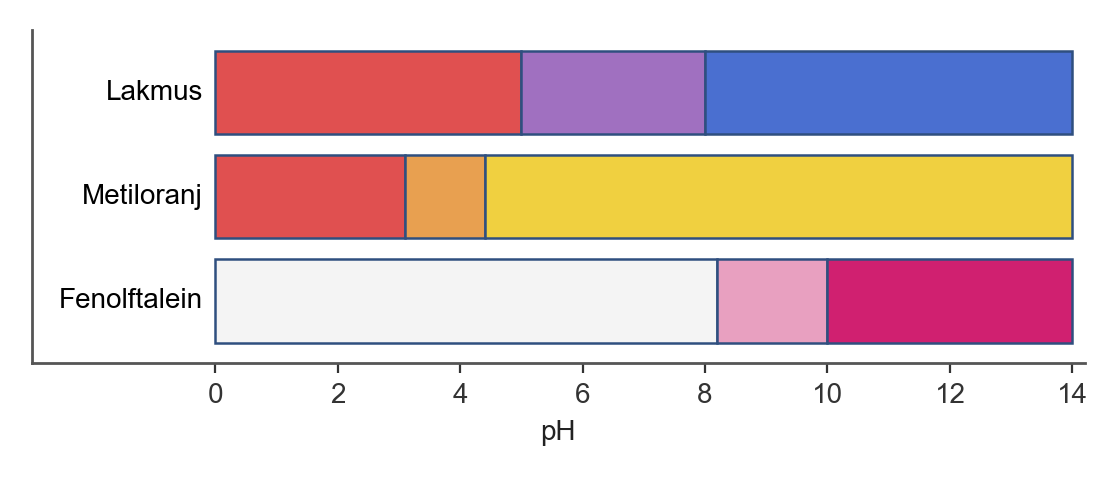
\includegraphics[width=0.86\linewidth]{rasmlar/gen/in_987786.png}\end{center}
pH = 11 bo`lgan eritmada fenolftalein qanday rangga kiradi?

\noindent\begin{tabular}{@{}p{0.47\linewidth}@{}p{0.47\linewidth}@{}}
A)~\textsl{malina rang} & B)~\textsl{rangsiz} \\
C)~\textsl{binafsha} & D)~\textsl{sariq} \\
\end{tabular}\par
\qsep
\noindent\qn{2.} 0,5 M H\textsubscript{3}PO\textsubscript{4} eritmasining normal \textbf{konsentratsiyasini (n) aniqlang.}

\noindent A)~\textsl{1,5} \hfill B)~\textsl{0,5} \hfill C)~\textsl{3} \hfill D)~\textsl{0,167}\par
\qsep
\noindent\qn{3.} Na\textsubscript{2}CO\textsubscript{3} eritmasida gidrolizlanish darajasini oshirish uchun qaysi usullar qo`llanadi? 1) qattiq Na\textsubscript{2}CO\textsubscript{3} qo`shib, konsentratsiyani oshirish; 2) sovitish; 3) NaOH eritmasi qo`shish; 4) NH\textsubscript{4}Cl eritmasi qo`shish

\noindent A)~\textsl{4} \hfill B)~\textsl{2, 3} \hfill C)~\textsl{1, 3} \hfill D)~\textsl{3}\par
\qsep
\noindent\qn{4.} Jadvalda bog`lar hosil qiluvchi atomlarning elektrmanfiyliklari berilgan:
\begin{center}
\renewcommand{\arraystretch}{1.15}
\fitbox{\begin{tabular}{|c|c|c|}\hline
\textbf{Bog`} & \textbf{EM (1-atom)} & \textbf{EM (2-atom)} \\ \hline
H--Cl & 2,1 & 3 \\ \hline
C--H & 2,5 & 2,1 \\ \hline
Mg--O & 1,2 & 3,5 \\ \hline
H--O & 2,1 & 3,5 \\ \hline
\end{tabular}}
\end{center}
Qaysi bog` eng qutbli (eng ko`p ionli xarakterga ega)?

\noindent A)~\textsl{Mg--O} \hfill B)~\textsl{H--Cl} \hfill C)~\textsl{C--H} \hfill D)~\textsl{H--O}\par
\qsep
\noindent\qn{5.} 40 g NaOH 250 g suvda eritildi. Eritmaning molyal \textbf{konsentratsiyasini (mol/kg) aniqlang.}

\noindent A)~\textsl{3,45} \hfill B)~\textsl{0} \hfill C)~\textsl{4} \hfill D)~\textsl{8}\par
\qsep
\noindent\qn{6.} Jadvalda S elementining birikmalaridagi oksidlanish darajasi berilgan:
\begin{center}
\renewcommand{\arraystretch}{1.15}
\fitbox{\begin{tabular}{|c|c|}\hline
\textbf{Modda} & \textbf{Oksidlanish darajasi} \\ \hline
S & 0 \\ \hline
SO\textsubscript{3} & +6 \\ \hline
SO\textsubscript{2} & +4 \\ \hline
H\textsubscript{2}S & -2 \\ \hline
\end{tabular}}
\end{center}
Ushbu moddalardan nechtasida S elementi faqat qaytaruvchi xossani namoyon qiladi? (S uchun eng past oksidlanish darajasi -2, eng yuqorisi +6)

\noindent A)~\textsl{2} \hfill B)~\textsl{3} \hfill C)~\textsl{1} \hfill D)~\textsl{0}\par
\qsep
\noindent\qn{7.} NH\textsubscript{4}Cl eritmasida gidrolizlanish darajasini oshirish uchun qaysi usullar qo`llanadi? 1) qizdirish; 2) sovitish; 3) HCl qo`shish; 4) qattiq NH\textsubscript{4}Cl qo`shib, konsentratsiyani oshirish

\noindent A)~\textsl{2, 3} \hfill B)~\textsl{4} \hfill C)~\textsl{1} \hfill D)~\textsl{1, 2}\par
\qsep
\noindent\qn{8.} Faqat qaytaruvchi bo`la oladigan \textbf{ionlarni aniqlang}: 1) Zn\textsuperscript{2+}; 2) Fe\textsuperscript{3+}; 3) Al\textsuperscript{3+}; 4) I\textsuperscript{$-$}

\noindent A)~\textsl{1, 2} \hfill B)~\textsl{4} \hfill C)~\textsl{3} \hfill D)~\textsl{2, 3}\par
\qsep
\noindent\qn{9.} Na\textsubscript{2}SO\textsubscript{4}$\cdot$10H\textsubscript{2}O kristallogidratida kristallizatsion suvning massa \textbf{ulushini (\%) aniqlang.}

\noindent A)~\textsl{55,9} \hfill B)~\textsl{44,1} \hfill C)~\textsl{28} \hfill D)~\textsl{126,8}\par
\qsep
\noindent\qn{10.} Elementning massa-spektri (izotoplar tarqalganligi) berilgan.
\begin{center}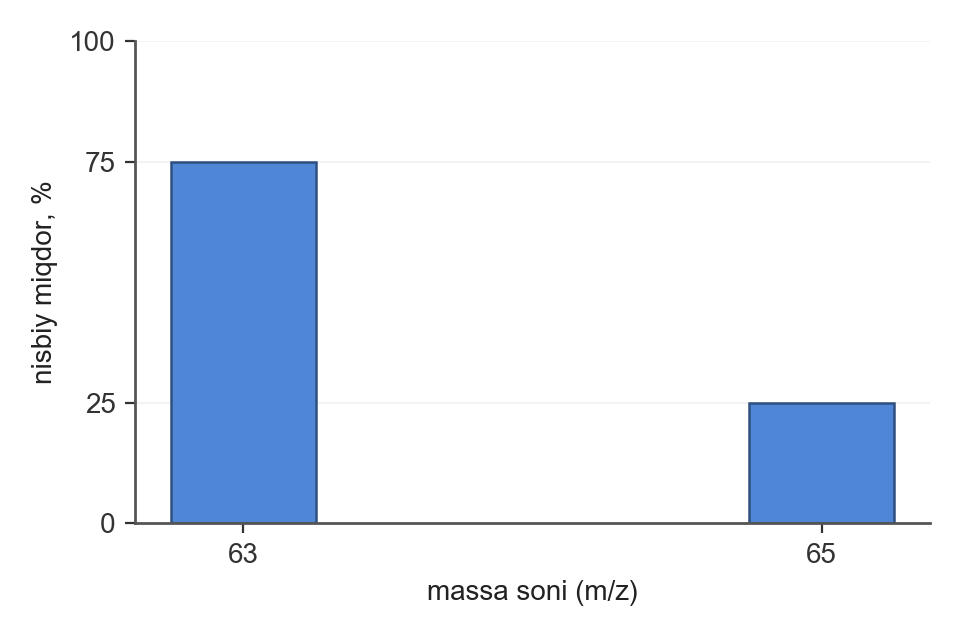
\includegraphics[width=0.86\linewidth]{rasmlar/gen/ms_v17_0.png}\end{center}
Elementning o`rtacha nisbiy atom \textbf{massasini aniqlang.}

\noindent A)~\textsl{64} \hfill B)~\textsl{63,5} \hfill C)~\textsl{64,5} \hfill D)~\textsl{63}\par
\qsep
\noindent\qn{11.} C\textsubscript{2}H\textsubscript{6} va NH\textsubscript{3} aralashmasi tarkibida aralashmadagi atomlarning umumiy soni 2,8$\cdot$N\textsubscript{A}. Aralashmaning massasi 11,1 g. Aralashmaning vodorodga nisbatan \textbf{zichligini aniqlang.}

\noindent A)~\textsl{22,2} \hfill B)~\textsl{5,55} \hfill C)~\textsl{15} \hfill D)~\textsl{11,1}\par
\qsep
\noindent\qn{12.} Jadvalda K\textsubscript{2}SO\textsubscript{4} ning ikki eritmasi haqida ma'lumot berilgan:
\begin{center}
\renewcommand{\arraystretch}{1.15}
\fitbox{\begin{tabular}{|c|c|c|}\hline
\textbf{Eritma} & \textbf{Massasi, g} & \textbf{Massa ulushi, \%} \\ \hline
1 & 100 & 15 \\ \hline
2 & 150 & 25 \\ \hline
\end{tabular}}
\end{center}
Eritmalar aralashtirilib, ustiga 50 g suv qo`shildi. Hosil bo`lgan eritmaning massa \textbf{ulushini (\%) aniqlang.}

\noindent A)~\textsl{20} \hfill B)~\textsl{40} \hfill C)~\textsl{19} \hfill D)~\textsl{17,5}\par
\qsep
\noindent\qn{13.} Na\textsubscript{2}CO\textsubscript{3} va MgCO\textsubscript{3} aralashmasi tarkibida Na\textsubscript{2}CO\textsubscript{3} ning massasi MgCO\textsubscript{3} ning massasidan 36,2 g ga ko`p. Shu aralashma mo`l xlorid kislota bilan ta'sirlashganda 15,68 l (n.sh.) gaz ajraldi. Reaksiyaga sarflangan HCl \textbf{miqdorini (mol) hisoblang.}

\noindent A)~\textsl{2,8} \hfill B)~\textsl{1,4} \hfill C)~\textsl{0,7} \hfill D)~\textsl{2,1}\par
\qsep
\noindent\qn{14.} Quyidagi mineral o`g`itlardan qaysilari fosforli o`g`itlar jumlasiga kiradi? 1) Ca(H\textsubscript{2}PO\textsubscript{4})\textsubscript{2}; 2) (NH\textsubscript{4})\textsubscript{2}SO\textsubscript{4}; 3) CO(NH\textsubscript{2})\textsubscript{2}; 4) Ca\textsubscript{3}(PO\textsubscript{4})\textsubscript{2}

\noindent A)~\textsl{1, 4} \hfill B)~\textsl{2} \hfill C)~\textsl{2, 3, 4} \hfill D)~\textsl{1, 3, 4}\par
\qsep
\noindent\qn{15.} 17 g NaNO\textsubscript{3} to`liq parchalanguncha qizdirildi. Qattiq qoldiq \textbf{massasini (g) aniqlang.}

\noindent A)~\textsl{17} \hfill B)~\textsl{27,6} \hfill C)~\textsl{13,8} \hfill D)~\textsl{6,9}\par
\qsep
\noindent\qn{16.} Probirkalardagi eritmalar: NaCl, Na\textsubscript{2}CO\textsubscript{3}, Na\textsubscript{2}SO\textsubscript{4} ni alohida probirkalarda ajratish uchun qaysi reagent(lar) yetarli? 1) BaCl\textsubscript{2}; 2) HCl va lakmus; 3) HCl va BaCl\textsubscript{2}; 4) BaCl\textsubscript{2} va fenolftalein

\noindent A)~\textsl{1, 4} \hfill B)~\textsl{1, 3} \hfill C)~\textsl{3, 4} \hfill D)~\textsl{3}\par
\qsep
\noindent\qn{17.} 6 mol H\textsubscript{2}S 6 mol kislorodda yondirildi (H\textsubscript{2}S to`liq sarflandi; oltingugurt va SO\textsubscript{2} aralashmasi hosil bo`ldi). Hosil bo`lgan oltingugurtning \textbf{massasini (g) hisoblang.}

\noindent A)~\textsl{192} \hfill B)~\textsl{96} \hfill C)~\textsl{48} \hfill D)~\textsl{144}\par
\qsep
\noindent\qn{18.} 4,8 g magniy havoda yondirilganda 7,6 g qattiq mahsulot hosil bo`ldi. Shu mahsulot mo`l suv bilan ishlanganda ajralgan ammiakning \textbf{hajmini (l, n.sh.) hisoblang.}

\noindent A)~\textsl{0,448} \hfill B)~\textsl{0,896} \hfill C)~\textsl{1,344} \hfill D)~\textsl{1,792}\par
\qsep
\noindent\qn{19.} 0,4 mol fosfat kislota 0,6 mol NaOH bilan ta'sirlashtirildi (reagentlar to`liq sarflandi). Hosil bo`lgan Na\textsubscript{2}HPO\textsubscript{4} \textbf{massasini (g) aniqlang.}

\noindent A)~\textsl{24} \hfill B)~\textsl{56,8} \hfill C)~\textsl{14,2} \hfill D)~\textsl{28,4}\par
\qsep
\noindent\qn{20.} Arenlar, neft va tabiiy gaz haqida qaysi fikrlar to`g`ri? 1) Tabiiy gazning asosiy qismi propan; 2) Neft fraksiyalaridan gazolin 150 \textdegree{}C gacha haydaladi; 3) Benzol uchun birikish reaksiyalari mutlaqo xos emas; 4) Benzoldan nitrobenzol nitrolash bilan olinadi

\noindent A)~\textsl{1, 2, 4} \hfill B)~\textsl{4} \hfill C)~\textsl{2, 4} \hfill D)~\textsl{1, 2}\par
\qsep
\noindent\qn{21.} Murakkab efirlar va yog`lar haqida qaysi fikrlar to`g`ri? 1) Dietil efir spirtdan yuqori haroratda qaynaydi; 2) Sovun --- yuqori yog` kislotalarning natriyli tuzi; 3) Suyuq yog`lar to`yinmagan kislotalardan hosil bo`lgan; 4) Murakkab efirlarning gidrolizi ishqoriy muhitda qaytmas

\noindent A)~\textsl{2, 4} \hfill B)~\textsl{2, 3, 4} \hfill C)~\textsl{1, 2, 4} \hfill D)~\textsl{3, 4}\par
\qsep
\noindent\qn{22.} Quyidagi birikmalardan qaysi biri aldegid sinfiga kiradi?

\noindent\begin{tabular}{@{}p{0.47\linewidth}@{}p{0.47\linewidth}@{}}
A)~\textsl{C\textsubscript{6}H\textsubscript{5}OH} & B)~\textsl{CH\textsubscript{3}COOC\textsubscript{2}H\textsubscript{5}} \\
C)~\textsl{C\textsubscript{2}H\textsubscript{5}NH\textsubscript{2}} & D)~\textsl{CH\textsubscript{3}CHO} \\
\end{tabular}\par
\qsep
\noindent\qn{23.} Formaldegid va butanal aralashmasi (13,8 g) mo`l ammiakli kumush oksid eritmasi bilan qizdirilganda 75,6 g kumush ajraldi. Reagent (ammiakli kumush oksid) eritmasining massa ulushi 36\% va zichligi 1,18 g/ml; u mo`l miqdorda olingan. Aralashmadagi butanalning \textbf{massasini (g) aniqlang.}

\noindent A)~\textsl{3} \hfill B)~\textsl{10,8} \hfill C)~\textsl{21,6} \hfill D)~\textsl{6,9}\par
\qsep
\noindent\qn{24.} 450 g glukoza spirtli bijg`ishga uchradi (unum 90\%). Reagent (ohakli suv) eritmasining massa ulushi 36\% va zichligi 1,12 g/ml; u mo`l miqdorda olingan. Ajralgan gaz mo`l ohakli suvdan o`tkazilganda necha gramm cho`kma hosil bo`ladi?

\noindent A)~\textsl{500} \hfill B)~\textsl{225} \hfill C)~\textsl{900} \hfill D)~\textsl{450}\par
\qsep
\noindent\qn{25.} Izobutan qizdirilib, quyidagi sxema bo`yicha parchalandi: C\textsubscript{4}H\textsubscript{10} $\to$ C\textsubscript{3}H\textsubscript{6} + CH\textsubscript{4}. Hosil bo`lgan gazlar aralashmasining vodorodga nisbatan zichligi 23,2 bo`lsa, izobutanning parchalanish \textbf{unumini (\%) aniqlang.}

\noindent A)~\textsl{12} \hfill B)~\textsl{75} \hfill C)~\textsl{50} \hfill D)~\textsl{25}\par
\qsep
\noindent\qn{26.} 46 g C\textsubscript{2}H\textsubscript{5}OH dan quyidagi sxema bo`yicha divinil kauchuk olindi: 2C\textsubscript{2}H\textsubscript{5}OH $\to$ CH\textsubscript{2}=CH--CH=CH\textsubscript{2} $\to$ (--CH\textsubscript{2}--CH=CH--CH\textsubscript{2}--)n. Bosqichlarning unumi ketma-ket 80\%, 50\% ni tashkil qiladi. Olingan divinil kauchuk \textbf{massasini (g) aniqlang.}

\noindent A)~\textsl{21,6} \hfill B)~\textsl{5,4} \hfill C)~\textsl{10,8} \hfill D)~\textsl{27}\par
\qsep
\noindent\qn{27.} CaC\textsubscript{2} dan quyidagi sxema bo`yicha 7,14 g anilin olindi: CaC\textsubscript{2} $\to$ C\textsubscript{2}H\textsubscript{2} $\to$ C\textsubscript{6}H\textsubscript{6} $\to$ C\textsubscript{6}H\textsubscript{5}NO\textsubscript{2} $\to$ C\textsubscript{6}H\textsubscript{5}NH\textsubscript{2}. Bosqichlarning unumi ketma-ket 40\%, 90\%, 40\%, 40\% ni tashkil qiladi. Sarflangan CaC\textsubscript{2} massasi (g) \textbf{ni aniqlang.}

\noindent A)~\textsl{256} \hfill B)~\textsl{512} \hfill C)~\textsl{128} \hfill D)~\textsl{102,4}\par
\qsep
\noindent\qn{28.} Chumoli va sirka kislota aralashmasi mo`l NaHCO\textsubscript{3} eritmasi bilan ta'sirlashganda 8,96 l (n.sh.) gaz ajraldi. Shu miqdordagi aralashma ammiakli kumush oksid bilan qizdirilganda 64,8 g kumush hosil bo`ldi. Qizdirish 45 daqiqa davom etdi. Reaksiyaga sarflangan NaHCO\textsubscript{3} \textbf{massasini (g) hisoblang.}

\noindent A)~\textsl{25,2} \hfill B)~\textsl{8,4} \hfill C)~\textsl{67,2} \hfill D)~\textsl{33,6}\par
\qsep
\noindent\qn{29.} 44,8 l (n.sh.) C\textsubscript{2}H\textsubscript{4} dan quyidagi sxema bo`yicha sirka kislota olindi: C\textsubscript{2}H\textsubscript{4} $\to$ C\textsubscript{2}H\textsubscript{5}OH $\to$ CH\textsubscript{3}CHO $\to$ CH\textsubscript{3}COOH. Bosqichlarning unumi ketma-ket 80\%, 90\%, 90\% ni tashkil qiladi. Olingan sirka kislota \textbf{massasini (g) aniqlang.}

\noindent A)~\textsl{77,76} \hfill B)~\textsl{155,52} \hfill C)~\textsl{38,88} \hfill D)~\textsl{86,4}\par
\qsep
\noindent\qn{30.} Rasmdagi tajribada cho`g`langan yog`och konsentrlangan HNO\textsubscript{3} bug`lari ichida yonmoqda. Bu jarayonda HNO\textsubscript{3} qanday vazifani bajaradi?
\begin{center}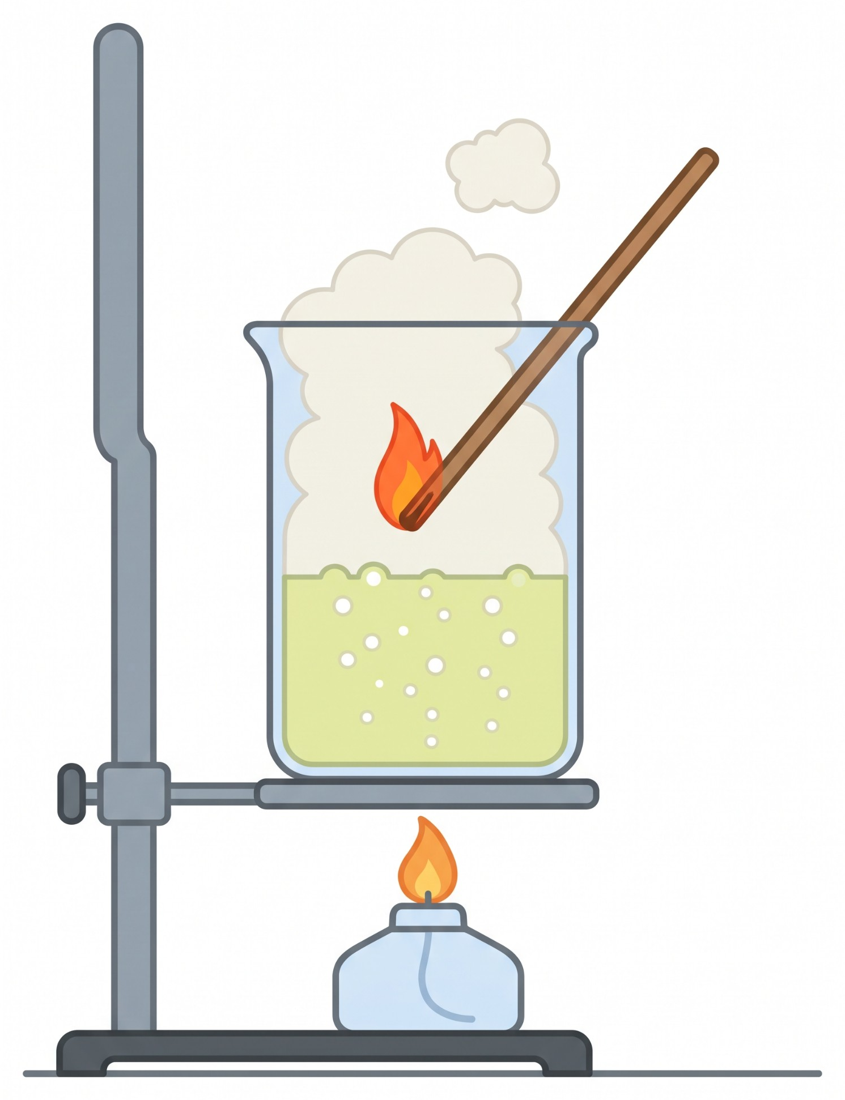
\includegraphics[width=0.86\linewidth]{rasmlar/darslik/d_hno3_yogoch.png}\end{center}

\noindent\begin{tabular}{@{}p{0.47\linewidth}@{}p{0.47\linewidth}@{}}
A)~\textsl{katalizator} & B)~\textsl{erituvchi} \\
C)~\textsl{qaytaruvchi} & D)~\textsl{oksidlovchi} \\
\end{tabular}\par
\qsep
\noindent\qn{31.} Quyidagi aralashmalarni ajratish usullarini mos qatorda \textbf{ko`rsating.} Aralashmalar: 1) loyqa suv (suv va gil); 2) etanol va suv; 3) temir va oltingugurt kukunlari. Usullar: a) tindirish va filtrlash; b) suvda eritish, filtrlash, bug`latish; c) magnit yordamida; d) fraksiyalab haydash.

\noindent\begin{tabular}{@{}p{0.47\linewidth}@{}p{0.47\linewidth}@{}}
A)~\textsl{1-c, 2-a, 3-d} & B)~\textsl{1-a, 2-d, 3-c} \\
C)~\textsl{1-c, 2-d, 3-a} & D)~\textsl{1-a, 2-c, 3-d} \\
\end{tabular}\par
\qsep
\noindent\qn{32.} Metiloranj indikatori kislotali muhitda qanday rang beradi?
\noindent A)~\textsl{ko`k}\par
\noindent B)~\textsl{rangsiz}\par
\noindent C)~\textsl{qizil}\par
\noindent D)~\textsl{malina rangga kiradi (pushti)   ---}\par
\qsep
\end{multicols}
\medskip
\noindent\setlength{\fboxsep}{0pt}\fbox{\begin{tabular}{p{0.74\linewidth}|p{0.2\linewidth}}
\parbox[t]{0.72\linewidth}{\vspace{3pt}\textbf{Topshiriqlar (33--35) va javob variant (A--F)larini o`zaro to`g`ri moslashtiring.} 25 g CuSO\textsubscript{4}$\cdot$5H\textsubscript{2}O suvda eritilib, hajmi 1000 ml bo`lgan eritma tayyorlandi. Eritma inert elektrodlar yordamida 5 A tok kuchi bilan 1930 s elektroliz qilindi (eritma hajmi o`zgarmadi deb hisoblang). Elektrolizdan keyin eritmaga mo`l NaOH qo`shilib, hosil bo`lgan cho`kma ajratildi, qizdirildi, so`ng hosil bo`lgan qattiq modda vodorod oqimida to`liq qaytarildi.
\vspace{3pt}} & \parbox[t]{0.19\linewidth}{\vspace{3pt}A~\textsl{0,8}\\[3pt]
B~\textsl{0,08}\\[3pt]
C~\textsl{1}\\[3pt]
D~\textsl{2}\\[3pt]
E~\textsl{0,1}\\[3pt]
F~\textsl{3,2}}\\ \hline
\parbox[t]{0.72\linewidth}{\vspace{2pt}\textbf{33. Dastlabki eritmada CuSO\textsubscript{4} ning molyar konsentratsiyasini (mol/l) hisoblang.}\vspace{2pt}} & \\ \hline
\parbox[t]{0.72\linewidth}{\vspace{2pt}\textbf{34. Elektroliz tugagach eritmaning pH ini aniqlang.}\vspace{2pt}} & \\ \hline
\parbox[t]{0.72\linewidth}{\vspace{2pt}\textbf{35. Oxirida olingan metall massasini (g) toping.}\vspace{2pt}} & 
\end{tabular}}
\par\bigskip
\noindent\qn{36.} Cu + HNO\textsubscript{3} $\to$ Cu(NO\textsubscript{3})\textsubscript{2} + NO + H\textsubscript{2}O reaksiya tenglamasini tenglang va barcha koeffitsiyentlar \textbf{yig`indisini aniqlang.} Tajriba 20 daqiqa davom etdi.
\javob\qsep
\noindent\qn{37.} CO + H\textsubscript{2}O $\rightleftarrows$ CO\textsubscript{2} + H\textsubscript{2} sistemasida boshlang`ich moddalarning har biridan 1 mol dan 5 l hajmli idishga solindi. Muvozanat qaror topganda reagentlarning har birining 3/5 qismi sarflangan bo`ldi. Tajriba laboratoriyada, kvars idishda o`tkazildi. Muvozanat \textbf{konstantasini hisoblang.}
\javob\qsep
\noindent\qn{38.} N\textsubscript{2}O\textsubscript{4} $\rightleftarrows$ 2NO\textsubscript{2} reaksiyasi doimiy harorat va bosimda olib borildi; boshlang`ich modda qisman o`zgargach gazlar hajmi 7/4 marta ortdi. Tajriba 40 daqiqa davom etdi. Boshlang`ich modda necha foizi \textbf{o`zgarganini aniqlang.}
\javob\qsep
\noindent\qn{39.} Bir asosli to`yingan karbon kislotaning 36 g miqdori mo`l NaHCO\textsubscript{3} bilan ta'sirlashganda 13,44 l (n.sh.) gaz ajraldi. Shu kislotaning 2/3 qismi mo`l etanol bilan esterlandi (efir unumi 1/2). Barcha reaksiyalar 1,5 atm bosimda olib borildi. Hosil bo`lgan murakkab efirning \textbf{massasini (g) toping.}
\javob\qsep
\noindent\qn{40.} Bir asosli to`yingan karbon kislotaning 52,8 g miqdori mo`l NaHCO\textsubscript{3} bilan ta'sirlashganda 13,44 l (n.sh.) gaz ajraldi. Shu kislotaning 2/3 qismi mo`l etanol bilan esterlandi (efir unumi 4/5). Barcha reaksiyalar 2 atm bosimda olib borildi. Hosil bo`lgan murakkab efirning \textbf{massasini (g) toping.}
\javob\qsep
\par\bigskip\begin{center}\textbf{\fontsize{13}{15}\selectfont YOZMA ISH}\end{center}
\noindent\qn{41.} \textbf{Topshiriqni bajarish jarayonida barcha reaksiya tenglamalarini yozing. Miqdoriy va arifmetik hisoblashlarni (unga asos bo`lgan usul yoki formulani ko`rsatgan holda) uzviy ketma-ketlikda bajaring.}\par\smallskip
KX (\textit{X} -- galogen) tuzining 11,9 g namunasi mo`l AgNO\textsubscript{3} eritmasi bilan ta'sirlashganda hosil bo`lgan cho`kma massasi tuz massasidan 1,58 marta katta bo`ldi. Xuddi shunday massadagi KX namunasi MnO\textsubscript{2} va sulfat kislota bilan qizdirilib, ajralgan oddiy modda vodorod bilan to`liq reaksiyaga kiritildi, hosil bo`lgan gaz 200 g suvda eritildi. Reagent (AgNO\textsubscript{3}) eritmasining massa ulushi 50\% va zichligi 1,3 g/ml; u mo`l miqdorda olingan. Olingan eritma 10\% li NaOH eritmasi bilan to`liq neytrallandi.\par
\noindent 1)\ KX ning AgNO\textsubscript{3} bilan reaksiyasi tenglamasini yozing va nisbatdan foydalanib \textit{X} galogenni aniqlang.\par
\noindent 2)\ KX ni MnO\textsubscript{2} va H\textsubscript{2}SO\textsubscript{4} bilan oksidlash reaksiyasini yozing; ajralgan oddiy moddaning massasini (g) va sarflangan MnO\textsubscript{2} massasini (g) hisoblang.\par
\noindent 3)\ Oddiy modda vodorod bilan reaksiyaga kirishganda hosil bo`lgan HX massasini (g) va uning suvdagi eritmasida massa ulushini (\%) toping.\par
\noindent 4)\ Neytrallash uchun sarflangan 10\% li NaOH eritmasining massasini (g) aniqlang.\par
\noindent 5)\ Neytrallangan eritmadagi NaX ning massa ulushini (\%) hisoblang.\par
\diqqat{Mazkur topshiriq kengaytirilgan javobni talab etib, uning yechilish usuli va shu usul asosidagi barcha hisoblash amallari javoblar varaqasida aks etishi lozim.}\qsep
\noindent\qn{42.} Organik moddalarning xossalarini bilgan holda reaksiya tenglamalarini tugallang va tenglashtiring. 3- va 5-reaksiyalarda hosil bo`lgan asosiy organik mahsulotlarni sistematik nomenklatura bo`yicha nomlang. Hosil bo`lgan organik moddalarning tuzilish formulalarini yozing.\par
\noindent 1)\ 2CH\textsubscript{3}--CH\textsubscript{2}--OH (H\textsubscript{2}SO\textsubscript{4} kons., 140 \textdegree{}C) $\to$\par
\noindent 2)\ CH\textsubscript{3}--CH\textsubscript{2}--CHO + Ag\textsubscript{2}O (NH\textsubscript{3}, t) $\to$\par
\noindent 3)\ C\textsubscript{6}H\textsubscript{5}--NO\textsubscript{2} + H\textsubscript{2} (Ni, t) $\to$\par
\noindent 4)\ C\textsubscript{6}H\textsubscript{5}--CH\textsubscript{3} + Cl\textsubscript{2} (yorug`lik) $\to$\par
\noindent 5)\ CH$\equiv$CH + H\textsubscript{2}O (Hg\textsuperscript{2+}, H\textsuperscript{+}) $\to$\par
\noindent 6)\ C\textsubscript{6}H\textsubscript{5}--OH + Br\textsubscript{2} (suvli eritma) $\to$\par
\noindent 7)\ 2CH\textsubscript{3}--Cl + 2Na $\to$\par
\diqqat{Mazkur topshiriq kengaytirilgan javobni talab etib, uning yechilish usuli va shu usul asosidagi barcha hisoblash amallari javoblar varaqasida aks etishi lozim.}\qsep
\noindent\qn{43.} \textbf{Topshiriqni bajarish jarayonida barcha reaksiya tenglamalarini yozing. Miqdoriy va arifmetik hisoblashlarni (unga asos bo`lgan usul yoki formulani ko`rsatgan holda) uzviy ketma-ketlikda bajaring.}\par\smallskip
NO\textsubscript{2} va O\textsubscript{2} aralashmasi (27 \textdegree{}C, 83,14 kPa da hajmi 48 l) 500 g suvga yuborildi. Yutilmay qolgan gaz hajmi shu sharoitda 6 l bo`ldi. R = 8,314 J/(mol$\cdot$K). Olingan nitrat kislota eritmasiga stexiometrik miqdorda CaCO\textsubscript{3} qo`shildi, hosil bo`lgan tuz eritmasi bug`latilib, qoldiq doimiy massagacha qizdirildi, ajralgan gazlar suvga yuttirildi.\par
\noindent 1)\ Reaksiya tenglamalarini yozing va qaysi gaz ortiqcha bo`lganini aniqlang.\par
\noindent 2)\ Dastlabki aralashmadagi NO\textsubscript{2} va O\textsubscript{2} ning mol miqdorlarini hamda hajmiy ulushlarini (\%) toping.\par
\noindent 3)\ Hosil bo`lgan eritmadagi HNO\textsubscript{3} ning massasini (g) va massa ulushini (\%) hisoblang. Kislotani neytrallash uchun sarflangan CaCO\textsubscript{3} massasini (g) va ajralgan CO\textsubscript{2} hajmini (l, n.sh.) toping.\par
\noindent 4)\ Dastlabki aralashmadagi NO\textsubscript{2} va O\textsubscript{2} ning massalarini (g) toping. Bug`latib qizdirilgandan keyin qolgan qattiq moddaning massasini (g) hisoblang.\par
\noindent 5)\ Dastlabki aralashmaning havoga nisbatan zichligini (M(havo) = 29 g/mol) aniqlang. Ajralgan gazlar suvga yuttirilganda qayta hosil bo`lgan HNO\textsubscript{3} massasini (g) aniqlang.\par
\diqqat{Mazkur topshiriq kengaytirilgan javobni talab etib, uning yechilish usuli va shu usul asosidagi barcha hisoblash amallari javoblar varaqasida aks etishi lozim.}\qsep
\newpage
\noindent\textbf{\fontsize{13}{15}\selectfont 17-variant}\hfill \textbf{Javoblar kaliti}\par\smallskip\hrule\smallskip
\textit{Faqat o`qituvchi uchun.}\par\medskip
\noindent\textbf{1--32-savollar}\par\smallskip
\noindent\begin{tabular}{|c|c|c|c|c|c|c|c|c|c|c|c|c|c|c|c|}\hline
\textbf{1} & \textbf{2} & \textbf{3} & \textbf{4} & \textbf{5} & \textbf{6} & \textbf{7} & \textbf{8} & \textbf{9} & \textbf{10} & \textbf{11} & \textbf{12} & \textbf{13} & \textbf{14} & \textbf{15} & \textbf{16}\\\hline
\textsl{A} & \textsl{A} & \textsl{A} & \textsl{A} & \textsl{C} & \textsl{C} & \textsl{C} & \textsl{B} & \textsl{A} & \textsl{B} & \textsl{D} & \textsl{D} & \textsl{B} & \textsl{A} & \textsl{C} & \textsl{C}\\\hline
\textbf{17} & \textbf{18} & \textbf{19} & \textbf{20} & \textbf{21} & \textbf{22} & \textbf{23} & \textbf{24} & \textbf{25} & \textbf{26} & \textbf{27} & \textbf{28} & \textbf{29} & \textbf{30} & \textbf{31} & \textbf{32}\\\hline
\textsl{B} & \textsl{B} & \textsl{D} & \textsl{C} & \textsl{B} & \textsl{D} & \textsl{B} & \textsl{D} & \textsl{D} & \textsl{C} & \textsl{A} & \textsl{D} & \textsl{A} & \textsl{D} & \textsl{B} & \textsl{C}\\\hline
\end{tabular}\par\medskip
\noindent\textbf{33--35-savollar}\par\smallskip
\noindent\begin{tabular}{|c|c|c|}\hline \textbf{No} & \textbf{Javob} & \textbf{Qiymat}\\\hline
33 & \textsl{E} & 0,1\\\hline
34 & \textsl{C} & 1\\\hline
35 & \textsl{F} & 3,2\\\hline
\end{tabular}\par\medskip
\noindent\textbf{36--40-savollar}\par\smallskip
\noindent\begin{tabular}{|c|c|}\hline \textbf{No} & \textbf{To`g`ri javob}\\\hline
36 & 20\\\hline
37 & 2,25\\\hline
38 & 75\\\hline
39 & 17,6\\\hline
40 & 37,12\\\hline
\end{tabular}\par\medskip
\noindent\textbf{41--43-topshiriqlar: javoblar}\par\smallskip
\noindent\textbf{41-topshiriq.}\par
\noindent 1) Br\par
\noindent 2) 8 g; 4,35 g\par
\noindent 3) 8,1 g; 3,89\%\par
\noindent 4) 40 g\par
\noindent 5) 4,15\%\par
\noindent\textbf{42-topshiriq.}\par
\noindent 1) 2CH\textsubscript{3}--CH\textsubscript{2}--OH $\to$ CH\textsubscript{3}--CH\textsubscript{2}--O--CH\textsubscript{2}--CH\textsubscript{3} + H\textsubscript{2}O\par
\noindent 2) CH\textsubscript{3}--CH\textsubscript{2}--CHO + Ag\textsubscript{2}O $\to$ CH\textsubscript{3}--CH\textsubscript{2}--COOH + 2Ag$\downarrow$\par
\noindent 3) C\textsubscript{6}H\textsubscript{5}--NO\textsubscript{2} + 3H\textsubscript{2} $\to$ C\textsubscript{6}H\textsubscript{5}--NH\textsubscript{2} + 2H\textsubscript{2}O --- nomi: \textbf{anilin}\par
\noindent 4) C\textsubscript{6}H\textsubscript{5}--CH\textsubscript{3} + Cl\textsubscript{2} $\to$ C\textsubscript{6}H\textsubscript{5}--CH\textsubscript{2}Cl + HCl\par
\noindent 5) CH$\equiv$CH + H\textsubscript{2}O $\to$ CH\textsubscript{3}--CHO --- nomi: \textbf{etanal}\par
\noindent 6) C\textsubscript{6}H\textsubscript{5}--OH + 3Br\textsubscript{2} $\to$ C\textsubscript{6}H\textsubscript{2}Br\textsubscript{3}--OH$\downarrow$ + 3HBr\par
\noindent 7) 2CH\textsubscript{3}--Cl + 2Na $\to$ CH\textsubscript{3}--CH\textsubscript{3} + 2NaCl\par
\noindent\textbf{43-topshiriq.}\par
\noindent 1) NO\par
\noindent 2) 1,4 mol; 0,2 mol\par
\noindent 3) 13,39\%; 60 g; 13,44 l\par
\noindent 4) 64,4 g; 6,4 g; 33,6 g\par
\noindent 5) 1,53; 75,6 g\par
\par\bigskip\noindent\textbf{Mavzular taqsimoti}\par\smallskip
{\small\noindent\begin{longtable}{|c|p{7.2cm}|p{5.4cm}|c|}\hline \textbf{No} & \textbf{Mavzu} & \textbf{Tekshiriladigan ko`nikma} & \textbf{Ball}\\\hline
1 & 8-sinf (indikatorlar) & Rasm bo`yicha tahlil & 1\\\hline
2 & 11-sinf 4-bob (normal konsentratsiya) & Hisoblash va masala yechish & 1\\\hline
3 & 9-sinf; 11-sinf (tuzlar gidrolizi; Le-Shatelye) & Bilim va tushunish & 1\\\hline
4 & 8-sinf (kimyoviy bog`lanish turlari, jadval) & Jadval tahlili & 1\\\hline
5 & 11-sinf 4-bob (molyal konsentratsiya) & Hisoblash va masala yechish & 1\\\hline
6 & Tirkashev \textit{V} bob (OQR, jadval) & Jadval tahlili & 1\\\hline
7 & 9-sinf; 11-sinf (tuzlar gidrolizi; Le-Shatelye) & Bilim va tushunish & 1\\\hline
8 & Tirkashev \textit{V} bob; 11-sinf 7-bob & Bilim va tushunish & 1\\\hline
9 & 7-sinf; Tirkashev (kristallogidrat) & Hisoblash va masala yechish & 1\\\hline
10 & 8-sinf (izotoplar, massa-spektr) & Grafik tahlili & 1\\\hline
11 & 8-9-sinf (gaz aralashmalari; Avogadro qonuni) & Hisoblash va masala yechish & 1\\\hline
12 & Tirkashev III bob (eritmalar, jadval) & Jadval tahlili & 1\\\hline
13 & 8-9-sinf (karbonatlar; kislotalar bilan reaksiya) & Hisoblash va masala yechish & 1\\\hline
14 & Tashev (mineral o`g`itlar) & Bilim va tushunish & 1\\\hline
15 & Tashev (nitratlar termik parchalanishi) & Hisoblash va masala yechish & 1\\\hline
16 & 9-sinf (ion reaksiyalar, anionlarni aniqlash) & Bilim va tushunish & 1\\\hline
17 & 9-sinf (vodorod sulfidning yonishi) & Hisoblash va masala yechish & 1\\\hline
18 & 9-sinf (magniyning yonishi; nitridlar) & Hisoblash va masala yechish & 1\\\hline
19 & 9-sinf (ko`p negizli kislotalar, nordon tuzlar) & Hisoblash va masala yechish & 1\\\hline
20 & 10-sinf (mavzuga oid paragraflar); Abdusamatov & Bilim va tushunish & 1\\\hline
21 & 10-sinf (mavzuga oid paragraflar); Abdusamatov & Bilim va tushunish & 1\\\hline
22 & 10-sinf (organik birikmalar sinflari) & Bilim va tushunish & 1\\\hline
23 & 10-sinf (aldegidlarning kumush ko`zgu reaksiyasi) & Hisoblash va masala yechish & 1\\\hline
24 & 10-sinf (uglevodlar; glukozaning bijg`ishi) & Hisoblash va masala yechish & 1\\\hline
25 & 10-sinf (alkanlarning krekingi va degidrogenlanishi) & Hisoblash va masala yechish & 1\\\hline
26 & 10-sinf (Lebedev usuli) & Hisoblash va masala yechish & 1\\\hline
27 & 10-sinf (karbiddan atsetilen, benzol, anilin) & Hisoblash va masala yechish & 1\\\hline
28 & 10-sinf (karbon kislotalar; chumoli kislotaning o`ziga xosligi) & Hisoblash va masala yechish & 1\\\hline
29 & 10-sinf (alkenlar, spirtlar, aldegidlar, kislotalar) & Hisoblash va masala yechish & 1\\\hline
30 & 8-sinf (nitrat kislota, 28-rasm) & Rasm bo`yicha tahlil & 1\\\hline
31 & 7-sinf (aralashmalarni ajratish); kimyoviy tahlil & Bilim va tushunish & 1\\\hline
32 & 8-sinf (indikatorlar) & Bilim va tushunish & 1\\\hline
33--35 & Aralash masala (moslashtirish) & Ko`p bosqichli hisob & 3\\\hline
36--40 & Qisqa javobli masalalar & Hisoblash & 5\\\hline
41--43 & Yozma ish & Usul va hisob (M, A) & 75\\\hline
\end{longtable}}
\end{document}
